\documentclass[main]{subfiles}


\newcommand{\grad}{\hspace{-2mm}$\phantom{a}^{\circ}$}
\newcommand{\degc}{$^\circ$C}
\begin{document}


\chapter{Magnetómetro}
\label{chap:magnetometro}

\section{Objetivos}

El objetivo de estas pruebas es comprender y caracterizar el magnetómetro de 3 ejes Honeywell HMC5583, incorporado para asistir en la determinación de la orientación absoluta del cuadricóptero.

\section{Materiales}
\label{sec:materiales}

\begin{itemize}
\item Mesa de madera de 1.5m de largo.
\item Laptop.
\item Hilo y clavos.
\item Mesa nivelable.
\item Cubo de lapacho
\item IMU ``Mongoose'' de CKDevices, con un HMC5583.
\item Foto satelital, con información sobre coordenadas.
\item Mesa nivelable, con una superficie que se pueda inclinar en ángulos conocidos.
\item Escuadra
\end{itemize}

\newpage

\section{Procedimiento}
\label{sec:procedimiento}

El modelo adoptado para relacionar las medidas de campo magnético sin calibrar con las medidas calibradas es idéntico al utilizado a la hora de calibrar el acelerómetro y el giróscopo. Se trata de realizar una transformación lineal de las medidas obtenidas para transformarlas en los valores de campo magnético. Se propone un modelo de la forma:
$$
\mathbf{C^p} =K_m (\mathbf{\tilde{C^m}} -  \mathbf{b_m})
$$

Se proponen dos métodos de calibración. En primer lugar se toman medidas de campo magnético con la plataforma alineada en una dirección conocida, sobre una mesa nivelada (de forma que se encuentre paralela a la superficie de la Tierra). Se toman las medidas del campo magnético variando el ángulo de la mesa y rotando la plataforma ángulos conocidos. Finalmente realizando una minimización por mínimos cuadrados se determinan los parámetros de interés.  

Por otra parte, se toma una serie de medidas de campo magnético terrestre en la mayor cantidad de  orientaciones posibles. Para asegurar la calidad de los datos es recomendable tomar medidas distribuidas uniformemente en todas las direcciones. Dado que el campo es constante, la gráfica de las medidas anteriores debería resultar en una esfera con centro en el origen de radio igual al módulo del campo magnético de la Tierra. Al no tener un sensor calibrado el resultado será un elipsoide. Se utilizó un algoritmo desarrollado por \emph{Alain Barraud} para realizar la calibración, dicho algoritmo no es otra cosa que la implementación de la minimización presente en el método propuesto por \ref{bib:Merayo}. El resultado que se obtiene es la matriz y el vector que hacen que las medidas tomadas aproximen una esfera de centro el origen.\\

Una vez calibrado el sensor se procede a verificar la exactitud que ofrece el mismo para determinar la orientación de la plataforma. Con dicho objetivo 
Cabe aclarar que el Norte magn\'etico no se corresponde con el Norte geogr\'afico en toda la Tierra, sino que por el contrario (dependiendo de la regi\'on del mundo) presenta una declinaci\'on. Es decir que tenemos una componente del campo magn\'etico en la dirección Oeste-Este adem\'as de la componente Sur-Norte. La declinaci\'on es diferente en cada punto de la 
Tierra. En particular en Uruguay la misma es de $-9.74^{\circ}$ seg\'un la convenci\'on mundial, es decir que el Norte magn\'etico se encuentra $9.74^{\circ}$ al Oeste del Norte geogr\'afico. 

\section{Resultados y Análisis}

\subsection{Calibración con el primer método}

Con el primer método propuesto se obtuvieron los siguientes resultados:

\begin{itemize}
\item $K_m=\left(\begin{array}{ccc}
      7.24\times10^{-4}   &  -2.79\times10^{-5}  &   -2.63\times10^{-5}\\
      8.03\times10^{-5}   &  7.23\times10^{-4}   &   1.89\times10^{-5}\\
      6.19\times10^{-5}   &  -5.07\times10^{-5}  &    7.80\times10^{-4}\\
	
\end{array}  \right)$
\item $\mathbf{b_m}= \left( \begin{array}{c}
  32.990198627287\\
           -120.1211527671\\
           4.6285537022096\\
\end{array}\right)
$
\item Error promedio: $ \mu = -1.07\times10^{8} G$\\
\item Desviación estándar: $\sigma =0.014 G$
\end{itemize}

Si bien el error promedio parece aceptable la desviación estándar no lo es. El valor del campo magnético en Uruguay en la dirección Norte es de $0.175 G$. La desviación estándar corresponde al $8\%$ del valor del campo magnético. En las demás direcciones el error cometido será aún mayor.\\


\subsection{Calibración con el segundo método}
Con el segundo método de calibración se obtienen los siguientes parámetros:
\begin{itemize}


\item $K_m=\left( \begin{array}{ccc}
 4.73\times10^{-3}   &  -2.19\times10^{-5}    &  3.09\times10^{-4} \\
                         0      & 4.55\times10^{-3}   &   7.83\times10^{-5} \\
                         0     &                    0   &    5.35\times10^{-3} \\
\end{array}
\right)
$

\item $
\mathbf{b_m}=\left(\begin{array}{c}
	23.32\\
	-126.62\\
    19.04
\end{array}\right)
$
\end{itemize}

\subsection{Primera Comparación entre los métodos}
En la figura \ref{fig:bola} se observan graficadas las medidas de campo magnético con el sensor descalibrado en los ejes solidarios a la plataforma. Como era de esperarse en la medida con el sensor descalibrado no se obtiene una esfera, esto se debe a que las ganancias en cada eje no son las adecuadas. Por otra parte los ejes principales tampoco son colineales con $X_q, Y_q $ y $ Z_q$. Debido a los \emph{offset} en cada dirección el centro del elipsoide no concuerda con el origen. En la figura \ref{fig:bolacalib} tenemos las medidas de campo magnético con el sensor calibrado con el segundo método de calibración propuesto. En primer lugar es interesante destacar que se tiene una esfera centrada en el origen, por lo tanto la calibración puede calificarse de exitosa. La magnitud que medimos luego del proceso de calibración se encuentra normalizada. Dado que utilizaremos dicho sensor para determinar una orientación, nos interesan simplemente las relaciones entre las componentes medidas en cada eje del sensor, por lo tanto trabajar con las medidas normalizadas arroja el mismo resultado que trabajar con las medidas de campo en Teslas o Gauss.\\

En la figura \ref{fig:bolanuestra} se transformaron las medidas utilizadas para realizar el segundo método de calibración utilizando los parámetros obtenidos gracias al primer método. Luego se normalizó el resultado obtenido a fin de poder compararlo con el resultado obtenido gracias al segundo método de calibración. Gráficamente no resulta evidente extraer una conclusión sobre cual de las dos medidas es más adecuada. 


\begin{figure}
  \begin{center}
	\subfloat[Con el sensor descalibrado]{\label{fig:bola}
	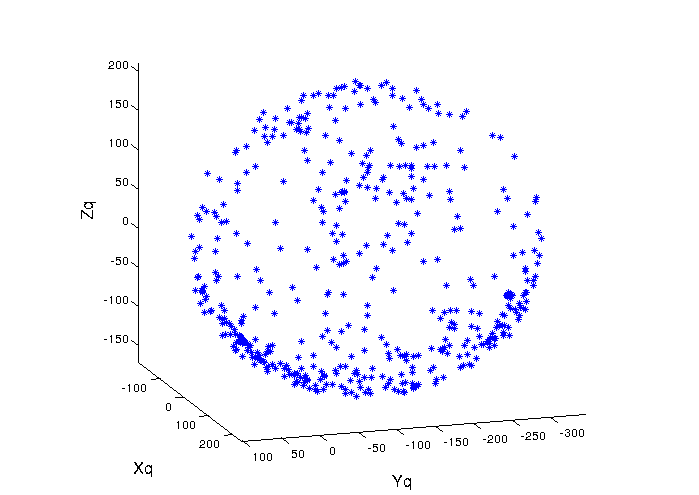
\includegraphics[width=0.35\textwidth]
		{./pics_magneto/bola.png}}
	\subfloat[Con el sensor calibrado]{\label{fig:bolacalib}
	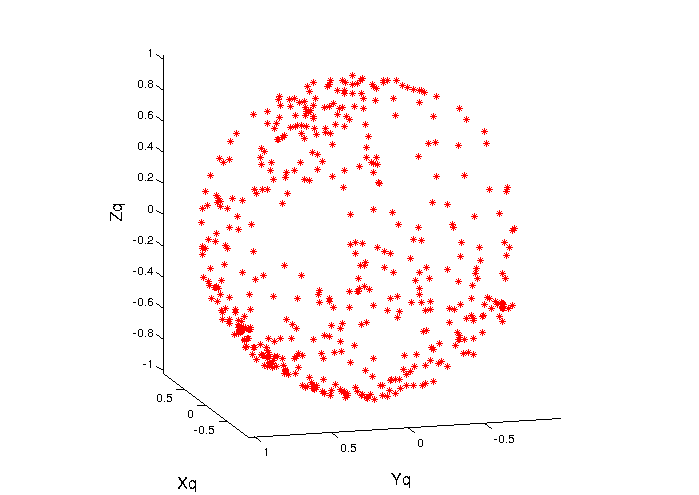
\includegraphics[width=0.35\textwidth]
		{./pics_magneto/bolacalib.png}}
	\subfloat[Con el sensor calibrado]{\label{fig:bolanuestra}
	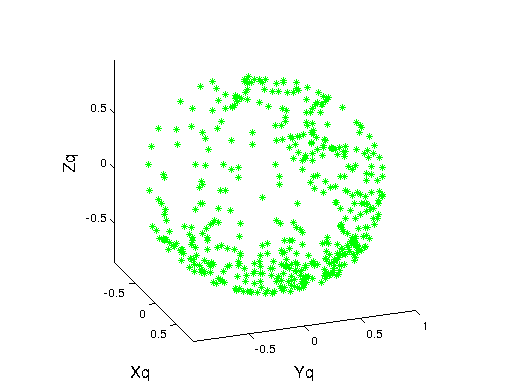
\includegraphics[width=0.35\textwidth]
		{./pics_magneto/bolanuestra.png}}
  \end{center}
  \caption{Medias de campo magnético Terrestre}
\end{figure}


Con los datos convertidos se procede a realizar una minimización gracias a los mínimos cuadrados para obtener las coordenadas del centro de cada esfera y su radio.

Para el primer método de calibración utilizado se encuentra que:
\begin{itemize}
\item Centro de la esfera: $C=(-3.86\times10^{-2};-6.53\times10^{-3};-5.99\times10^{-2})$
\item Radio de la esfera: $R=0.9389$
\item Error promedio: $\mu = -6.85\times10^{-4}$
\item Desviación estándar de la medida del radio: $\sigma = 3.55\times10^{-2}$
\end{itemize}

Para el segundo método de calibración utilizado se encuentra que:
\begin{itemize}
\item Centro de la esfera: $(2.39\times10^{-3};-2.63\times10^{-3};-5.38\times10^{-4})$
\item Radio de la esfera: $0.9979$
\item Error promedio: $\mu =-3.00\times 10^{-4}$
\item Desviación estándar de la medida del radio:$\sigma = 2.42\times 10^{-2}$
\end{itemize}


Si bien la diferencia obtenida entre ambas calibraciones no es significativa en cuanto a los errores cometidos en el radio de las esferas, sí aparece una diferencia de un orden de magnitud en una de las coordenadas del centro de la esfera y de dos ordenes de magnitud en otro. 


\subsection{Determinaci\'on de la orientaci\'on}
Luego de calibrado el sensor se quiere determinar la capacidad que tiene el mismo de proporcionar una adecuada orientación. Con dicho fin se utiliza la tabla larga para alinear el sensor en una dirección en particular. La ubicación donde fue realizado el experimento se encuentra marcada aproximadamente con la marca roja en la figura \ref{fig:mapa}. El objeto elegido para realizar la alineación es el que se muestra en la parte superior de la figura \ref{fig:mapa}, su ubicación es la indicada por el ``mu\~neco'' en la figura \ref{fig:mapa}.
\begin{figure}
  \begin{center}
	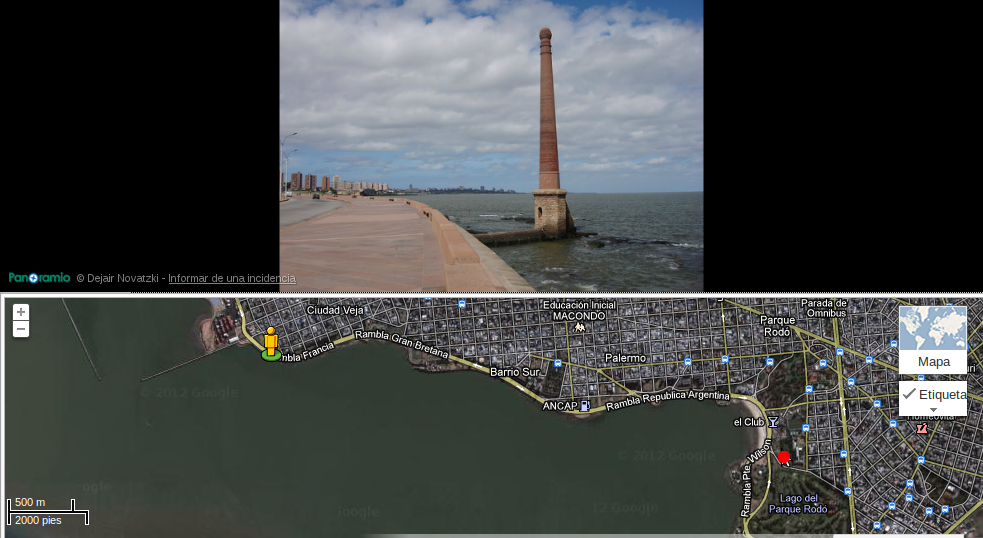
\includegraphics[width=0.8\textwidth]
		{./pics_magneto/mapa.png}
	
  \end{center}
  \caption{Mapa de la costa de Montevideo}
  \label{fig:mapa}
\end{figure}

Del mapa de la Intendencia de Montevideo \footnote{http://sig.montevideo.gub.uy/mapas/mapa-principal} se obtienen las coordenadas de los puntos seleccionados. El punto en que fue realizado el experimento es el (576039,6135625) y el punto con el cual se alineo es el (572118,6136415). El ángulo de la recta que une los dos puntos medido respecto del eje Sur-Norte es de $78.6^\circ$ al Oeste.\\

Interesa determinar los tres \'angulos de Euler ($\theta$, $\varphi$ y $\psi$). En primer lugar se intenta utilizando exclusivamente el magnet\'ometro. En las tablas \ref{tab:angulos} se presentan los resultados obtenidos para cada m\'etodo de calibraci\'on. En la tabla se observa claramente que los resultados difieren considerablemente de lo esperado. Se confirma que el magnet\'ometro por si solo, no es suficiente para determinar la orientaci\'on del cuadric\'optero. 

En reposo, los \'angulos de pitch y roll, pueden determinarse f\'acilmente gracias a la medida de aceleraci\'on. Luego de determinados dichos \'angulos se proyecta la lectura del campo magn\'etico en la base $S_1$ definida en \ref{chap:modelo_fisico}. La orientaci\'on se calcula finalmente como:

$$
\theta=atan(\vec{C_{med}}\vec{i_1}/\vec{C_{med}}\vec{j_1})
$$

Donde $C_{med}$ es el campo magn\'etico medido luego de proyectado en la base $S_1$. 

Los resultados obtenidos en este caso se presentan en la tabla \ref{tab:angulosconacc}.\\






\begin{table}
\begin{tabular}{|p{50pt}|p{50pt}|p{50pt}|p{51pt}|p{50pt}|p{50pt}|}
\hline
  
\multicolumn{2}{|p{113pt}|}{\cellcolor[gray]{0.6} $\theta$}  
& \multicolumn{2}{|p{114pt}|}{\cellcolor[gray]{0.6} $\varphi$}
& \multicolumn{2}{|p{113pt}|}{\cellcolor[gray]{0.6} $\psi$} 
\\ \hline 
   
 \multicolumn{1}{|p{50pt}|}{\cellcolor[gray]{0.7} \textbf{\'angulo te\'orico }} 
& \multicolumn{1}{|p{50pt}|}{\cellcolor[gray]{0.8} \textbf{ángulo medido}}
& \multicolumn{1}{|p{50pt}|}{\cellcolor[gray]{0.7} \textbf{\'angulo te\'orico }} 
& \multicolumn{1}{|p{50pt}|}{\cellcolor[gray]{0.8} \textbf{ángulo medido}}
& \multicolumn{1}{|p{50pt}|}{\cellcolor[gray]{0.7} \textbf{\'angulo te\'orico }} 
& \multicolumn{1}{|p{50pt}|}{\cellcolor[gray]{0.8} \textbf{ángulo medido}}
\\ \hline

 -90.20&  16.17&-90.00& 54.88&  0.00&-54.23\\ \hline
 -60.20&  27.47&-90.00& 43.92&  0.00&-26.59\\ \hline
 -45.20&  31.96&-90.00& 38.77&  0.00&-13.86\\ \hline
 -30.20&  35.82&-90.00& 33.57&  0.00& -1.70\\ \hline
  -0.20&  43.41&-90.00& 22.75&  0.00& 22.86\\ \hline
  89.80&  62.34&-90.00& -7.55&  0.00& 76.77\\ \hline
 -90.20& -30.76& -0.00&-19.64& 90.00& 23.46\\ \hline
 -60.20& -43.24& -0.00&-20.10& 90.00& 42.72\\ \hline
 -45.20& -45.54& -0.00&-17.55& 90.00& 53.33\\ \hline
 -30.20& -44.20& -0.00&-14.35& 90.00& 63.15\\ \hline
  -0.20& -28.13& -0.00& -9.57& 90.00& 79.90\\ \hline
  89.80&  46.50& -0.00&  0.62& 90.00& 61.21\\ \hline
 179.80&  24.61& -0.00&-11.21&180.00& 84.50\\ \hline
-150.20&  -3.43& -0.00& -9.98&180.00& 84.68\\ \hline
-135.20& -18.96& -0.00& -9.27&180.00& 85.06\\ \hline
-120.20& -33.05& -0.00& -8.56&180.00& 85.22\\ \hline
 -90.20& -63.76& -0.00& -6.57&180.00& 85.84\\ \hline
  -0.20&-156.62& -0.00&-15.41&180.00& 77.69\\ \hline
\end{tabular}
\caption{Ángulos medidos con la primer calibración y teóricos en las distintas posiciones}


\begin{tabular}{|p{50pt}|p{50pt}|p{50pt}|p{51pt}|p{50pt}|p{50pt}|}
\hline
  
\multicolumn{2}{|p{113pt}|}{\cellcolor[gray]{0.6} $\theta$}  
& \multicolumn{2}{|p{114pt}|}{\cellcolor[gray]{0.6} $\varphi$}
& \multicolumn{2}{|p{113pt}|}{\cellcolor[gray]{0.6} $\psi$} 
\\ \hline 
   

 \multicolumn{1}{|p{50pt}|}{\cellcolor[gray]{0.7} \textbf{\'angulo te\'orico }} 
& \multicolumn{1}{|p{50pt}|}{\cellcolor[gray]{0.8} \textbf{ángulo medido}}
& \multicolumn{1}{|p{50pt}|}{\cellcolor[gray]{0.7} \textbf{\'angulo te\'orico }} 
& \multicolumn{1}{|p{50pt}|}{\cellcolor[gray]{0.8} \textbf{ángulo medido}}
& \multicolumn{1}{|p{50pt}|}{\cellcolor[gray]{0.7} \textbf{\'angulo te\'orico }} 
& \multicolumn{1}{|p{50pt}|}{\cellcolor[gray]{0.8} \textbf{ángulo medido}}
\\ \hline

 -90.20&  22.89&-90.00& 62.86&  0.00&-50.24\\ \hline
 -60.20&  34.83&-90.00& 50.00&  0.00&-22.52\\ \hline
 -45.20&  39.31&-90.00& 44.14&  0.00&-10.21\\ \hline
 -30.20&  43.11&-90.00& 38.26&  0.00&  1.50\\ \hline
  -0.20&  50.58&-90.00& 25.49&  0.00& 25.90\\ \hline
  89.80&  60.40&-90.00&-12.45&  0.00& 83.52\\ \hline
 -90.20& -24.09& -0.00&-16.70& 90.00& 19.61\\ \hline
 -60.20& -36.79& -0.00&-18.84& 90.00& 38.91\\ \hline
 -45.20& -39.90& -0.00&-17.07& 90.00& 49.95\\ \hline
 -30.20& -39.70& -0.00&-14.39& 90.00& 60.29\\ \hline
  -0.20& -26.81& -0.00& -9.76& 90.00& 78.48\\ \hline
  89.80&  49.40& -0.00& -1.47& 90.00& 65.71\\ \hline
 179.80&  22.33& -0.00&-12.36&180.00& 88.71\\ \hline
-150.20&  -4.33& -0.00&-10.00&180.00& 85.71\\ \hline
-135.20& -18.88& -0.00& -9.31&180.00& 84.54\\ \hline
-120.20& -31.82& -0.00& -8.90&180.00& 83.65\\ \hline
 -90.20& -59.48& -0.00& -7.79&180.00& 83.71\\ \hline
  -0.20&-136.17& -0.00&  0.59&180.00& 84.91\\ \hline
\end{tabular}
\caption{Ángulos medidos con la segunda calibración y teóricos en las distintas posiciones}
\label{tab:angulos}
\end{table} 

\begin{table}
\begin{tabular}{|p{50pt}|p{50pt}|p{50pt}|p{51pt}|p{50pt}|p{50pt}|}
\hline
  
\multicolumn{2}{|p{113pt}|}{\cellcolor[gray]{0.6} $\theta$}  
& \multicolumn{2}{|p{114pt}|}{\cellcolor[gray]{0.6} $\varphi$}
& \multicolumn{2}{|p{113pt}|}{\cellcolor[gray]{0.6} $\psi$} 
\\ \hline 
   

 \multicolumn{1}{|p{50pt}|}{\cellcolor[gray]{0.7} \textbf{\'angulo te\'orico }} 
& \multicolumn{1}{|p{50pt}|}{\cellcolor[gray]{0.8} \textbf{ángulo medido}}
& \multicolumn{1}{|p{50pt}|}{\cellcolor[gray]{0.7} \textbf{\'angulo te\'orico }} 
& \multicolumn{1}{|p{50pt}|}{\cellcolor[gray]{0.8} \textbf{ángulo medido}}
& \multicolumn{1}{|p{50pt}|}{\cellcolor[gray]{0.7} \textbf{\'angulo te\'orico }} 
& \multicolumn{1}{|p{50pt}|}{\cellcolor[gray]{0.8} \textbf{ángulo medido}}
\\ \hline

-101.39&-102.65&-90.00&-90.00&  0.00&   0.00\\ \hline
 -71.39& -72.79&-90.00&-90.00&  0.00&   0.00\\ \hline
 -56.39& -58.60&-90.00&-90.00&  0.00&   0.00\\ \hline
 -41.39& -44.64&-90.00&-90.00&  0.00&   0.00\\ \hline
 -11.39& -15.33&-90.00&-90.00&  0.00&   0.00\\ \hline
  78.61&  65.13&-90.00&-90.00&  0.00&   0.00\\ \hline
-101.39&-100.11& -0.00& -2.21& 90.00&  92.22\\ \hline
 -71.39& -75.67& -0.00& -1.86& 90.00&  92.02\\ \hline
 -56.39& -63.05& -0.00& -1.72& 90.00&  91.97\\ \hline
 -41.39& -50.65& -0.00& -1.63& 90.00&  91.96\\ \hline
 -11.39& -23.03& -0.00& -1.55& 90.00&  92.24\\ \hline
  78.61&  70.92& -0.00& -1.41& 90.00&  93.40\\ \hline
 168.61& 165.02& -0.00& -0.11&180.00&-179.33\\ \hline
-161.39&-165.54& -0.00& -0.63&180.00&-179.59\\ \hline
-146.39&-149.33& -0.00& -0.73&180.00&-179.78\\ \hline
-131.39&-134.53& -0.00& -0.72&180.00& 179.94\\ \hline
-101.39&-102.08& -0.00& -0.57&180.00& 179.84\\ \hline
 -11.39& -16.00& -0.00& -0.02&180.00& 179.66\\ \hline
\end{tabular}
\caption{Ángulos medidos con la primer calibración y teóricos en las distintas posiciones, asistido por el aceler\'ometro}


\begin{tabular}{|p{50pt}|p{50pt}|p{50pt}|p{51pt}|p{50pt}|p{50pt}|}
\hline
  
\multicolumn{2}{|p{113pt}|}{\cellcolor[gray]{0.6} $\theta$}  
& \multicolumn{2}{|p{114pt}|}{\cellcolor[gray]{0.6} $\varphi$}
& \multicolumn{2}{|p{113pt}|}{\cellcolor[gray]{0.6} $\psi$} 
\\ \hline 
   

 \multicolumn{1}{|p{50pt}|}{\cellcolor[gray]{0.7} \textbf{\'angulo te\'orico }} 
& \multicolumn{1}{|p{50pt}|}{\cellcolor[gray]{0.8} \textbf{ángulo medido}}
& \multicolumn{1}{|p{50pt}|}{\cellcolor[gray]{0.7} \textbf{\'angulo te\'orico }} 
& \multicolumn{1}{|p{50pt}|}{\cellcolor[gray]{0.8} \textbf{ángulo medido}}
& \multicolumn{1}{|p{50pt}|}{\cellcolor[gray]{0.7} \textbf{\'angulo te\'orico }} 
& \multicolumn{1}{|p{50pt}|}{\cellcolor[gray]{0.8} \textbf{ángulo medido}}
\\ \hline

-101.39&-110.21&-90.00&-90.00&  0.00&   0.00\\ \hline
 -71.39& -77.27&-90.00&-90.00&  0.00&   0.00\\ \hline
 -56.39& -62.03&-90.00&-90.00&  0.00&   0.00\\ \hline
 -41.39& -47.03&-90.00&-90.00&  0.00&   0.00\\ \hline
 -11.39& -14.40&-90.00&-90.00&  0.00&   0.00\\ \hline
  78.61&  73.61&-90.00&-90.00&  0.00&   0.00\\ \hline
-101.39&-108.27& -0.00& -2.21& 90.00&  92.22\\ \hline
 -71.39& -80.63& -0.00& -1.86& 90.00&  92.02\\ \hline
 -56.39& -66.41& -0.00& -1.72& 90.00&  91.97\\ \hline
 -41.39& -52.67& -0.00& -1.63& 90.00&  91.96\\ \hline
 -11.39& -23.42& -0.00& -1.55& 90.00&  92.24\\ \hline
  78.61&  66.18& -0.00& -1.41& 90.00&  93.40\\ \hline
 168.61& 165.14& -0.00& -0.11&180.00&-179.33\\ \hline
-161.39&-164.83& -0.00& -0.63&180.00&-179.59\\ \hline
-146.39&-149.40& -0.00& -0.73&180.00&-179.78\\ \hline
-131.39&-135.93& -0.00& -0.72&180.00& 179.94\\ \hline
-101.39&-107.43& -0.00& -0.57&180.00& 179.84\\ \hline
 -11.39& -22.85& -0.00& -0.02&180.00& 179.66\\ \hline
\end{tabular}
\caption{Ángulos medidos con la segunda calibración y teóricos en las distintas posiciones, asistido por el aceler\'ometro}
\label{tab:angulosacc}
\end{table} 

En este caso los \'angulos encontrados se asemejan en mayor medida a los resultados te\'oricos.  



El error promedio obtenido con el primer m\'etodo de calibraci\'on es $\mu_1=-61^\circ$, la desviación estándar obtenida es $\sigma_1=3.83^\circ$, mientras que para el segundo método de calibración tenemos que $\mu_2=-7.10^\circ$, la desviación estándar obtenida es $\sigma_2=3.28^\circ$.\\

Cabe aclarar que la exactitud de los resultados obtenidos para las seis primeras medidas en los \'angulos de pitch y roll, se debe a un ajuste realizado para cubrirse frente a la situaci\'on de \emph{gimbal lock}. El an\'alisis del error cometido en la medida de los \'angulos de pitch y roll puede encontrarse en el cap\'itulo \ref{chap:acelerometro}.\\



En ambos casos se obtiene un error promedio distinto de cero. Con cualquier método de ajuste que se elija se deberá restar a la medida realizada el error promedio. Lo más adecuado parece ser elegir el método que tiene una desviación estándar menor. Por dicho motivo volvemos a escoger el segundo método. 




\end{document}


